%\section{How to Conduct Bulk Job}
%====================================================================================

\section{What's Bulk Job} \label{sec:bulkjob}
 \scalerm has a functionality for bulk jobs that allows simultaneous multiple execution of independent runs.
This function is useful for the parameter-sweep experiment, the ensemble experiment in different initial conditions, the time-slice climate simulation, and so on.

The bulk job function can be used not only for model simulation (\verb|scale-rm|), but also for the generation of topographical data, land-use data, and initial/boundary data. Note that the generation of topographical/land-use data by this function is limited to the case without a topography copy function (See \ref{subsec:nest_topo}).

In the following explanation, an independent execution in the bulk job is called a ``sub-job.'' Three two-domain nesting experiments are taken up as an example. This set of experiments is imaged as three sub-jobs with different integration periods and centers of calculation domain. \nmitem{NUM_DOMAIN, PRC_DOMAINS, CONF_FILES} in \namelist{PARAM_LAUNCHER} in the file \verb|launch.conf| (refer to Section \ref{subsubsec:launch} ) must be the same in all configurations. The other settings, such as integration time, the scheme used, and the number of grids per MPI process, do not need to be the same among the sub-jobs.

\begin{figure}[t]
\begin{center}
  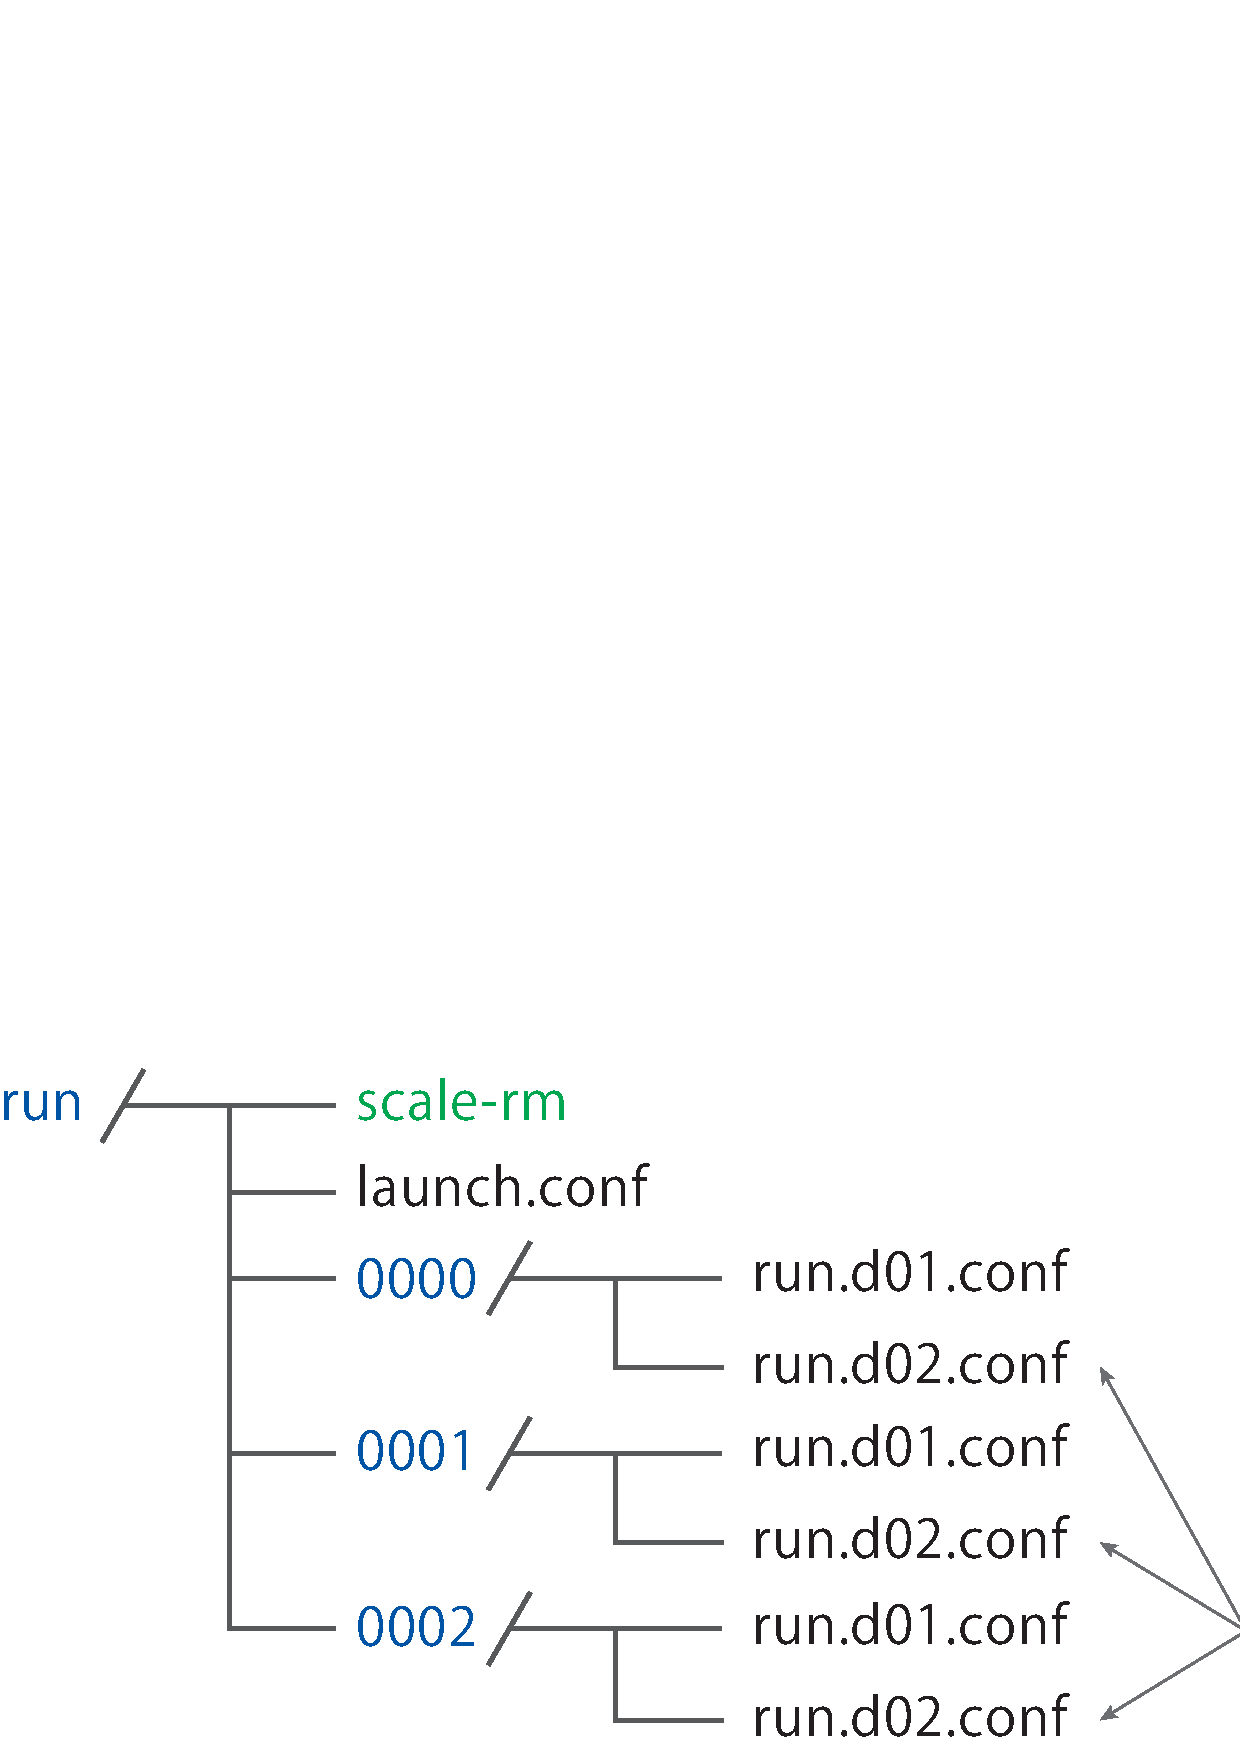
\includegraphics[width=0.6\hsize]{./../../figure/bulkjob_directory_structure.pdf}\\
  \caption{Structure of directories at the execution of \scalerm with bulk job.
Numbers such as ``0000'' are the directory names corresponding to job number, and called the job directory.   All necessary configuration files to execute sub jobs must be prepared in each job directory.
}
  \label{fig_bulkjob}
\end{center}
\end{figure}



\section{Settings for Bulk Job}
Since the bulk job function is an extension of the division and redistribution of MPI processes used in online nesting, file \verb|launch.conf| is required to launch the job. Even in case online nesting and bulk job functions are used together, only one file \verb|launch.conf| is prepared.
Below is an example of such a case.
\editboxtwo{
\verb|&PARAM_LAUNCHER|       & \\
\verb| NUM_BULKJOB = 3,|     & number of sub-jobs\\
\verb| NUM_DOMAIN  = 2,|     & number of nesting domains\\
\verb| PRC_DOMAINS = 9, 36,|  & number of total process in each domain\\
\verb| CONF_FILES  = run.d01.conf, run.d02.conf,| & name of configulation files\\
\verb| LOG_SPLIT   = .false.,| & log-output for mpi splitting?\\
\verb| COLOR_REORDER = .true.,| & coloring reorder for mpi splitting?\\
\verb| FAILURE_PRC_MANAGE = .false.,| & use failure process management?\\
\verb| NUM_FAIL_TOLERANCE = 1, | & tolerance number of failure processes\\
\verb| FREQ_FAIL_CHECK    = 5, | & FPM polling frequency per DT\\
\verb|/| \\
}
It is sufficient to add item \nmitem{NUM_BULKJOB} to the \verb|launch.conf|. The other configurations are similar to those in Section \ref{subsubsec:launch}. In case of a single-domain experiment (no nesting), specify \nmitem{NUM_DOMAIN} $=$ 1 and assign a file name to \nmitem{CONF_FILES}.

Log of MPI communicator splitting will be output, when \nmitem{LOG_SPLIT} is \verb|.true.|.
The default value of \nmitem{LOG_SPLIT} is \verb|.false.|.

Option of \nmitem{COLOR_REORDER} is the switch for job rearrangement in MPI communicator groups following the process size of the job. The job which has the largest process size is arranged at the front row;
this would be reasonable to gain the efficient inter-node communication.


\section{Failure Process Management}
In the \scalerm bulk job system, a failure process management (FPM) tool is available. FPM watches the job groups with a polling interval.
If some jobs are unfortunately aborted, all other jobs are not aborted until the number of failure jobs reaches to the limit number.
\nmitem{FAILURE_PRC_MANAGE} is a switch for use FPM tool.
\nmitem{NUM_FAIL_TOLERANCE} and \nmitem{FREQ_FAIL_CHECK} are setting parameters for limit number of failure jobs and interval of checking failure job, respectively.
Note, this version of FPM tool is available only for single domain calculation, not available of full system for online-nesting calculation. If you want to use FPM tool even in online-nesting calculation,
\nmitem{NUM_FAIL_TOLERANCE} must be equal to the number of all jobs.


\section{Preparation for Bulk Job}
Prior to the execution of bulk jobs, prepare as many directories as the number of sub-jobs, which are called ``sub-directories.'' As in Fig. \ref{fig_bulkjob}, these correspond to \verb|0000/  0001/  0002/|. The directory name is assigned as a four-digit number starting from zero. In each directory, all the necessary files (configuration files, input files, and output directories) must be prepared.
Note that the path to directories or files specified in the configuration files must be correctly set up as explained below.
An excerpt of \verb|run.d01.conf| for job \verb|0000| are as follows:
\editbox{
\verb|&PARAM_IO| \\
\verb| IO_LOG_BASENAME = "0000/LOG_d01",| \\
\verb|/| \\
 \\
\verb|&PARAM_RESTART| \\
\verb| RESTART_OUTPUT       = .true.,| \\
\verb| RESTART_OUT_BASENAME = "0000/restart_d01",| \\
\verb| RESTART_IN_BASENAME  = "../init/0000/init_d01_00013046400.000",| \\
\verb|/| \\
 \\
\verb|&PARAM_GRAPHY| \\
\verb| TOPOGRAPHY_IN_BASENAME = "../pp/0000/topo_d01",| \\
\verb|/| \\
 \\
\verb|&PARAM_LANDUSE| \\
\verb| LANDUSE_IN_BASENAME = "../pp/0000/landuse_d01",| \\
\verb|/| \\
 \\
\verb|&PARAM_ATMOS_BOUNDARY| \\
\verb| ~ ... ~             | \\
\verb| ATMOS_BOUNDARY_IN_BASENAME    = "../init/0000/boundary_d01",| \\
\verb| ~ ... ~             | \\
\verb|/                    | \\
 \\
\verb|&PARAM_FILE_HISTORY| \\
\verb| FILE_HISTORY_DEFAULT_BASENAME  = "0000/history_d01",| \\
\verb| ~ ... ~           | \\
\verb|/| \\
}

As shown in Fig. \ref{fig_bulkjob}, job directories exist in the same hierarchy as the directory of the executable binary. That is, a configuration file exists under each job directory, whereas the input files and the output directories must be described as relative paths from the location of  the executable binary. The output directory in the 0000 experiment is \verb|0000/| and the name of output files are as \verb|0000/***|. {\color{blue}{ Note that when the file name is common to all experiments without adding the name of job directory, the output is written to the same file, and the data disappear as a result.
}}


%% バルクジョブの実行は, 全サブジョブを実行するのに必要なMPIプロセス数を指定し,
%% \begin{verbatim}
%%  $ mpirun  -n  135  ./scale-rm  launch.conf
%% \end{verbatim}
%% と行う。例では, 一つのサブジョブあたり, $9 + 36 = 45$プロセス使用し, 全体で3つのジョブを実行するので,
%% 総計で135プロセスを必要とする。
%% %
%% 実行すると得られるLOGファイルに, MPIプロセスを分割した時の情報が示されている。
%% LOGファイルを開くと, 最初の「SCALEロゴ」のあとに下記のようなメッセージが出力される。
%% 下記, ドメイン1のプロセス0からの出力例である。\\


\section{Execution of Bulk Job}

At the execution of bulk jobs, the total number of MPI processes is specified as

\begin{verbatim}
 $ mpirun  -n  135  ./scale-rm  launch.conf
\end{verbatim}
In this example, the number of processes per sub-job is 45 ($=9 + 36$) and the total number of processes used for three sub-jobs is 135. The message providing information regarding the division of MPI processes is written to the LOG files after the \scalelib logo. The following example is the log output for process 0 of Domain 1:
\msgboxtwo{
\verb| +++++ start MPI|  & \\
\verb| *** UNIVERSAL_COMM_WORLD        :        0| &; different by execution environment\\
\verb| *** total process [UNIVERSAL]   :      135| &\\
\verb| *** my process ID [UNIVERSAL]   :       36| &\\
\verb| *** master rank?  [UNIVERSAL]   :        F| &\\
\verb| *** GLOBAL_COMM_WORLD           :        3| &; different by execution environment \\
\verb| *** total process [GLOBAL]      :       45| &\\
\verb| *** my process ID [GLOBAL]      :       36| &\\
\verb| *** master rank?  [GLOBAL]      :        F| &\\
\verb| *** LOCAL_COMM_WORLD            :        4| &; different by execution environment\\
\verb| *** total process [LOCAL]       :        9| &\\
\verb| *** my process ID [LOCAL]       :        0| &\\
\verb| *** master rank?  [LOCAL]       :        T| &\\
\verb| *** ABORT_COMM_WORLD            :        0| &\\
\verb| *** master rank ID [each world] :        0| &\\
&\\
}
The items belonging to \verb|[LOCAL]|, \verb|[GLOBAL]|, and \verb|[UNIVERSAL]| are the descriptions, respectively, of the process group in the domain, the nesting group, and the job group. The \verb|UNIVERSAL| group includes the \verb|GLOBAL| group and the \verb|GLOBAL| group includes the \verb|LOCAL| group. \verb|total process| represents the total number  of processes in each group and \verb|my process ID| is the ID of the process in the group.

It can be confirmed in this case that 1) since \verb|total process [UNIVERSAL]| is 135, all these processes are completed executed; 2) since \verb|total process [GLOBAL]| is 45, these 45 processes are used in a sub-job; 3) since the log file for Domain 1 is shown in this example, it is correct to describe \verb|total process [LOCAL]| as 9. If you see the log message for Domain 2,  it is 39. \verb|my process ID [UNIVERSAL]| is the process number  corresponding to the LOG and history files. Since this notation is the same as in the abnormal completion of execution, you can immediately recognize the processes in which errors occur during executing a considerable number of sub-jobs.


%%%%%%%%%%%%%%%%%%%%%%%%%%%%%%%%%%%%%%%%%%%%%%%%%%%%%%%%%%%%%%%%%%%%%%%%%%%%%%%%%%%%%%
